%-------------------------------------------------------------------------------------------------------------------
\section{Chemistry Workflow}
%-------------------------------------------------------------------------------------------------------------------

%-------------------------------------------------------------------------------------------------------------------
\begin{frame}

NU-WRF offers advanced aerosol modeling using the implementation of GOCART. This workflow is a incorporates steps from the  basic and the default workflow.However, it excludes the LIS steps and instead adds the GOCART2WRF preprocessor for providing chemical boundary conditions from GEOS-5 as well as the community PREP\_CHEM\_SOURCES program for emissions.  \\
\mbox{}\\
GOCART2WRF supports four possible sources of GOCART data:
\begin{itemize}
\item offline GOCART
\item on-line GOCART from GEOS5
\item MERRAero reanalyses
\item MERRA-2
\end{itemize}
\mbox{}\\
\emph{We will describe the "offline GOCART" case only.\\
LIS is not used.}
\mbox{}\\

\end{frame}

%-------------------------------------------------------------------------------------------------------------------
\begin{frame}

\centering
\textbf{NU-WRF chemistry workflow.}
\begin{figure}[t]
\centering
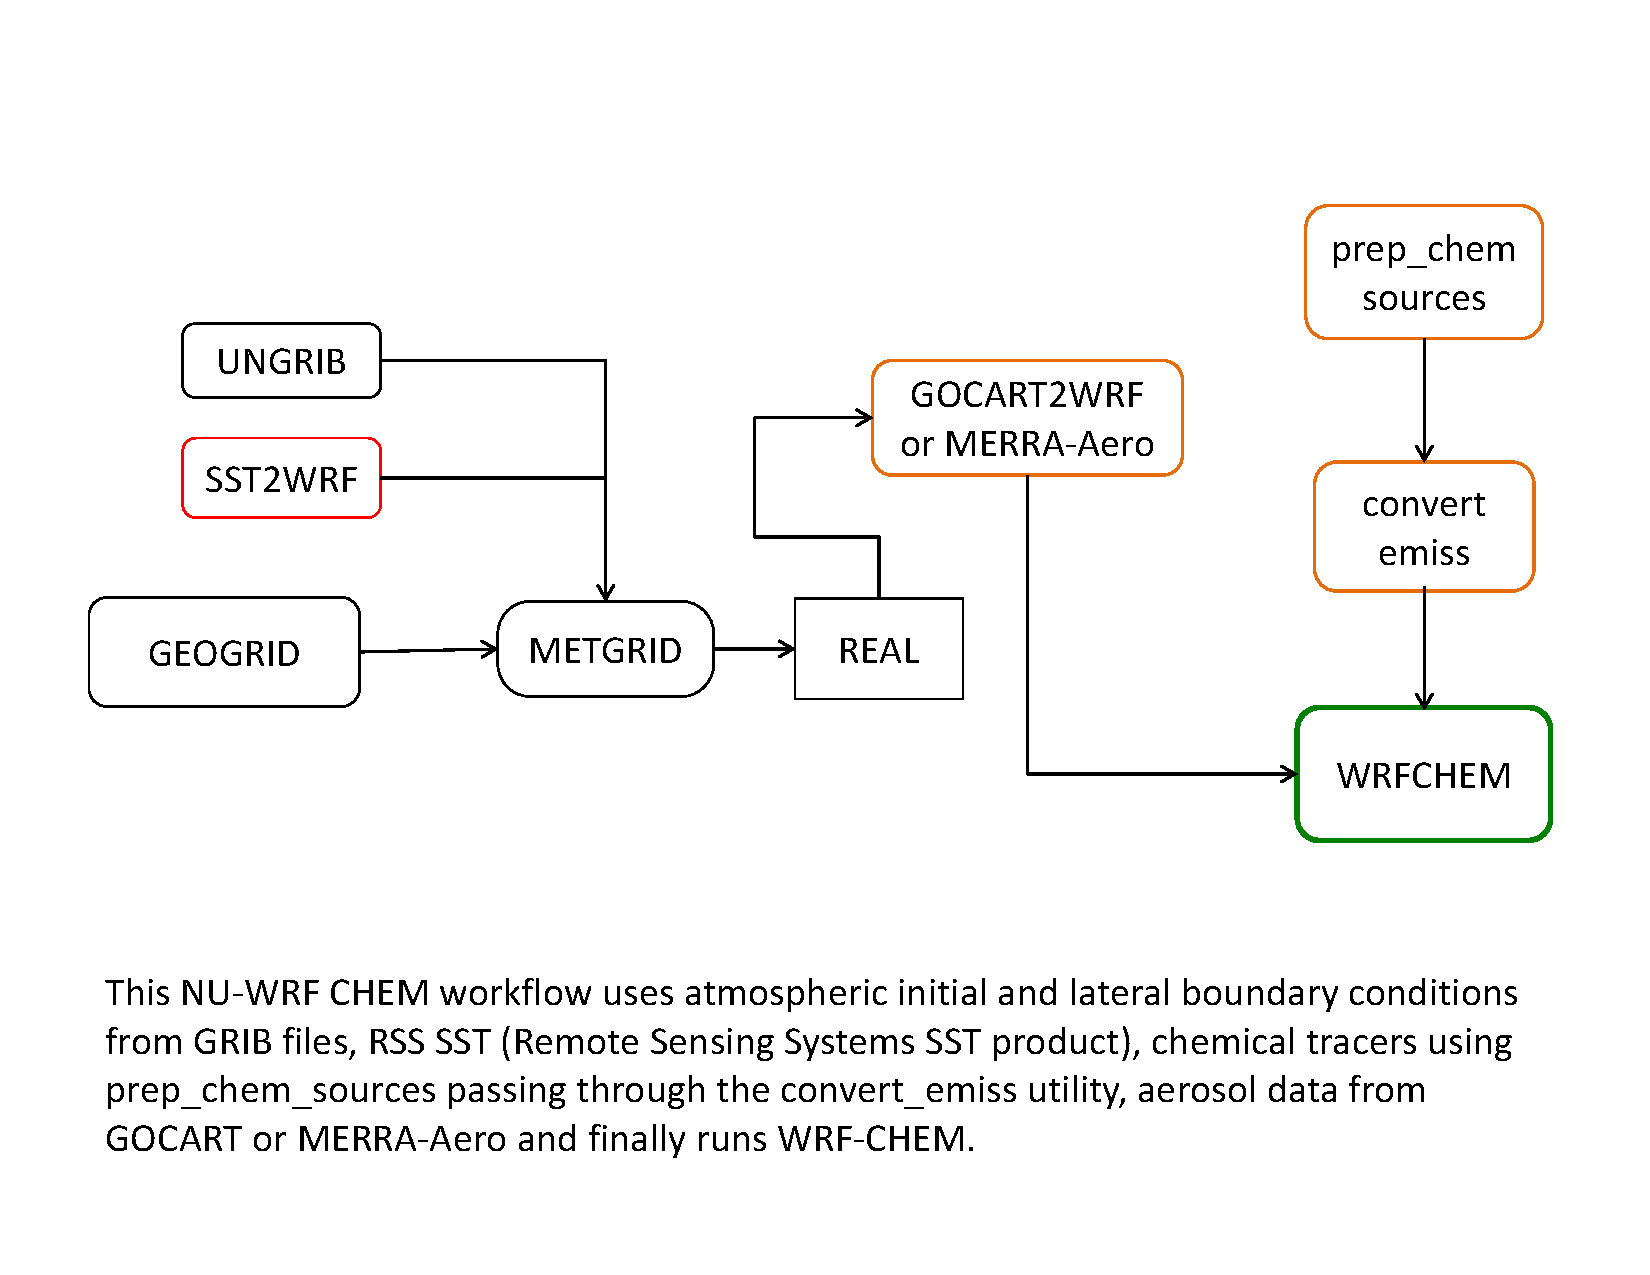
\includegraphics[scale=.4]{chemistry-workflow-1.pdf}
\end{figure}

\end{frame}

%-------------------------------------------------------------------------------------------------------------------
\begin{frame}[fragile]\frametitle{Required files for chemistry workflow}

Copy the following files to \textbf{RUNDIR}:
\begin{lstlisting}
> export RUNDIR=/discover/nobackup/<my_user_id>/scratch/chemistry_workflow
> cp -r $PROJECTDIR/tutorial/chemistry_workflow $RUNDIR

Where:
common.reg : shared script with settings used by other scripts.
*.reg : scripts to run pre-processors and model.
namelist* : namelist files required by executables.
data/ungrib : GRIB atmospheric data for initial conditions used by UNGRIB component.
data/gocart : data files used by GOCART
\end{lstlisting}

\end{frame}

%-------------------------------------------------------------------------------------------------------------------
\begin{frame}[fragile]
\frametitle{Required script changes}
\verbatimfont{\scriptsize}%
\begin{verbatim}
> cd $RUNDIR
\end{verbatim}
 Use your favorite editor to edit \textbf{common.reg} and change the values of NUWRFDIR and RUNDIR using the values set earlier.
\verbatimfont{\scriptsize}%
\begin{verbatim}
# *** Please make sure these settings are correct ***
# NUWRFDIR specifies the location of the NU-WRF source code
NUWRFDIR=<CHANGE THIS>
# RUNDIR specifies the location of the temporary run directory
RUNDIR=<CHANGE THIS>
\end{verbatim}
You may need to edit all the .reg files' account information and other settings. However, if you belong to group s0492 then the scripts should work without any modifications.
\verbatimfont{\scriptsize}%
\begin{verbatim}
Change account to appropriate SBU charge code:
#SBATCH --account s0942 
Change if you want to change number of nodes, hasw - to run on haswell nodes:
#SBATCH --ntasks=16 --constraint=hasw
Uncomment and set according to your needs and privileges:
##SBATCH --qos=high 
Uncomment (if desired) and substitute your e-mail here:
##SBATCH --mail-user=user@nasa.gov 
\end{verbatim}

\end{frame}

%-------------------------------------------------------------------------------------------------------------------
\begin{frame}[fragile]\frametitle{A note about namelists settings}

Things to keep in mind before we run NU-WRF components.
\mbox{}\\
\begin{itemize}
\item The length of the simulations is specified in the namelist files:
\begin{itemize}
\item In namelist.wps the length is determined by start\_date and end\_date
\item In namelist.input look for start\_ and end\_ fields. 
\item The dates in both namelists must be consistent.
\end{itemize}
\item The workflow is designed to work as-is. However, if you want to run for different dates:
\begin{itemize}
\item You must get the corresponding atmospheric data for initial conditions. 
\item You may need to modify the namelists. For example in namelist.input, make sure end\_day - start\_day = run\_days.
\end{itemize}
\item For \textbf{any} other changes please refer to the user's guide.
\end{itemize}

\end{frame}

%-------------------------------------------------------------------------------------------------------------------
\begin{frame}[fragile]\frametitle{GEOGRID}

\scriptsize{
GEOGRID interpolates static and climatological terrestrial data (land use, albedo, vegetation greenness, etc) to each WRF grid.
\begin{itemize}
\item Input: namelist.wps
\item Output: For \emph{N} domains (max\_dom in namelist.wps), \emph{N} geo\_em files will be created.
\end{itemize}\scriptsize}    
\hrulefill\par
\scriptsize{Before running GEOGRID ensure your domain is in the right location. To do so run plotgrids\_new.ncl}
\verbatimfont{\scriptsize}%
\begin{verbatim}
> module load other/ncl-6.3.0
> ncl $NUWRFDIR/WPS/util/plotgrids_new.ncl
\end{verbatim}
\scriptsize{This is where you would edit namelist.wps to modify the domain information.
Now run GEOGRID:}
\verbatimfont{\scriptsize}%
\begin{verbatim}
> cd $RUNDIR
> sbatch geogrid.reg
\end{verbatim}
When done, check for  "Successful completion"  string in the file geogrid.slurm.out.
geogrid.log.nnnn (nnnn is the cpu number) files will also be created for tracking run failures or debugging.

\end{frame}

%-------------------------------------------------------------------------------------------------------------------
\begin{frame}[fragile]\frametitle{UNGRIB}

\scriptsize{
UNGRIB unpacks GRIB1 or GRIB2 files that contain  meteorological data (soil moisture, soil temperature, sea surface temperature, sea ice, etc) and writes specific fields in a WPS intermediate format.
\begin{itemize}
\item Input: namelist.wps  and GRIB input data.
\item Output: Several NAM* files corresponding to number of intervals (interval\_seconds) in simulation length (start/end dates).
\end{itemize}}
\scriptsize{\textbf{Notes}: 
\begin{itemize}
\item The GRIB input is referenced in the run script, ungrib.reg:
      ./link\_grib.csh data/ungrib/nam*\\
\item The UNGRIB output (NAM) is determined by the settings in the WPS namelist (namelist.wps).
\item makes use of Vtables that list the fields and their GRIB codes that must be unpacked from the GRIB files.
\end{itemize}
}
\hrulefill\par
\scriptsize{To run:}
\verbatimfont{\scriptsize}%
\begin{verbatim}
> cd $RUNDIR
> ./ungrib.reg
\end{verbatim}
When done, check for "Successful completion" string in file ungrib\_logs/ungrib.log.

\end{frame}

%-------------------------------------------------------------------------------------------------------------------
\begin{frame}[fragile]
\frametitle{SST2WRF}

\footnotesize{
SST2WRF processes several sea surface temperature (SST) products produced by Remote Sensing Systems (RSS; see http://www.remss.com).\\
}    
\hrulefill\par
\footnotesize{To run:}
\begin{lstlisting}
> cd $RUNDIR
> ./sst2wrf.reg  # Not a batch script. It may take a few seconds to complete...

Example uses start date = 20090410 and end date = 20090411: 

When done, SSTRSS:* files will be created, and these files should be copied to the RUNDIR before running METGRID component. 

> cp $RUNDIR/sstdata/mw_ir/SSTRSS* $RUNDIR
\end{lstlisting}

\end{frame}


%-------------------------------------------------------------------------------------------------------------------
\begin{frame}[fragile]\frametitle{METGRID}

\footnotesize{
METGRID horizontally interpolates UNGRIB and SSTRSS output to the WRF domains, and combine them with the output from GEOGRID.
\begin{itemize}
\item Input: namelist.wps, geo\_em*, NAM*, and SSTRSS* files.
\item Output: Several met\_em* files corresponding to number of intervals (interval\_seconds) in simulation length (start/end dates).
\end{itemize}
}    
\hrulefill\par
\footnotesize{To run:}
\begin{lstlisting}
> cd $RUNDIR
> sbatch metgrid.reg
\end{lstlisting}
When done, check for  "Successful completion" string in the file metgrid.slurm.out. metgrid.log.nnnn (nnnn is the cpu number) files also be created for tracking run failures or debugging.


\end{frame}

%-------------------------------------------------------------------------------------------------------------------
\begin{frame}[fragile]\frametitle{REAL}

\footnotesize{
REAL vertically interpolates the METGRID output to the WRF grid, and creates initial and lateral boundary condition files.
\begin{itemize}
\item Input: namelist.input, met\_em*  files, geo\_em* files.
\item Output: wrfinput* files (one for each domain), wrfbdy\_d01.
\end{itemize}
}    
\hrulefill\par
\footnotesize{To run:}
\begin{lstlisting}
> cd $RUNDIR
> sbatch real.reg
\end{lstlisting}
Check real.slurm.out for run completion.
If necessary check the real\_logs directory for real.rsl.out.nnnn and real.rsl.error.nnnn files.


\end{frame}


%-------------------------------------------------------------------------------------------------------------------
\begin{frame}[fragile]\frametitle{GOCART2WRF}

\footnotesize{
GOCART2WRF extracts aerosol data from GEOS-5 netCDF4 GOCART files (or MERRA reanalysis aerosol data files); horizontally and vertically interpolates the fields to the WRF grid; and appends them to the initial and lateral boundary condition files of WRF (wrfinput\_d* and wrfbdy\_d01).  \\
User can choose GOCART aerosol data or MERRA reanalysis Aerosol data.  
\begin{itemize}
\item Input: namelist.gocart2wrf, grib\_input/*, wrfinput* files (one for each domain), wrfbdy\_d01.
\item Output: wrfinput* files (one for each domain), wrfbdy\_d01. Original wrfinput* and  wrfbdy\_d01 files will be backed up with .gocart2wrf extension.
\end{itemize}
}    
\hrulefill\par
\footnotesize{To run:}
\begin{lstlisting}
> cd $RUNDIR
>./gocart2wrf.reg  # runs in serial
\end{lstlisting}
Check this file for successful run completion: gc2wrf.log. 


\end{frame}

%-------------------------------------------------------------------------------------------------------------------
\begin{frame}[fragile]\frametitle{PREP\_CHEM\_SOURCES}

\footnotesize{
This community tool processes a number of biogenic, anthropogenic, volcanic, and wildfire emissions. The NU-WRF version has several modifications that are discussed in the user's guide. Running prep\_chem\_sources requires a prep\_chem\_sources.inp file and upon completion it produces map projection data (that can be visualized by plot\_chem) as well as other files used by convert\_emiss.
\begin{itemize}
\item Input: prep\_chem\_sources.inp
\item Output: nuwrf-T* files
\end{itemize}
}    
\hrulefill\par
\footnotesize{To run:}
\begin{lstlisting}
> cd $RUNDIR
> ./prep_chem_sources.reg   # runs in serial
\end{lstlisting}
Check this file for successful run completion: pcs.log. 

\end{frame}

%-------------------------------------------------------------------------------------------------------------------
\begin{frame}[fragile]\frametitle{Convert\_Emiss}

\footnotesize{
This is a community WRF-Chem preprocessor that takes the output from PREP CHEM SOURCES and rewrites the fields in new netCDF files for reading by WRF-Chem.
\begin{itemize}
\item Input: namelist.input.convert\_emiss files (one for each domain).
\item Output: wrfchemi\_gocart\_bg* and wrfchemi* files (one for each domain).
\end{itemize}
}    
\hrulefill\par
\footnotesize{To run:}
\begin{lstlisting}
> cd $RUNDIR
> sbatch convert_emiss.reg
\end{lstlisting}
Check ce.slurm.out  for run completion.


\end{frame}

%-------------------------------------------------------------------------------------------------------------------
\begin{frame}[fragile]\frametitle{WRF}

\footnotesize{
\hrulefill\par       
If we get to this point then we are ready to run WRF with chemistry.
\begin{itemize}
\item Input: namelist.input, wrfinput* files (one for each domain), wrfbdy\_d01, wrfchemi\_gocart\_bg* and wrfchemi* files.
\item Output: wrfout* files (one for each domain).
\end{itemize}
}    
\hrulefill\par
\footnotesize{To run:}
\begin{lstlisting}
> cd $RUNDIR
> sbatch wrf.reg
\end{lstlisting}
Check wrf.slurm.out for run completion.
If necessary check the wrf\_logs directory for wrf.rsl.out.nnnn and wrf.rsl.error.nnnn files.

\end{frame}

%-------------------------------------------------------------------------------------------------------------------
\begin{frame}[fragile]
\frametitle{Post-processing on Discover}

Using NCVIEW:

\begin{lstlisting}
WRF output files (NETCDF4) can be viewed using a special version of ncview installed on Discover:

/usr/local/other/SLES11.1/ncview/2.1.2/intel-12.1.0.233/bin/ncview <filename>
\end{lstlisting}

\end{frame}

%-------------------------------------------------------------------------------------------------------------------
\begin{frame}[fragile]
\frametitle{Post-processing on Discover}

Using RIP (NCAR graphics). Submit the \textbf{rip} job:
\begin{lstlisting}
> cd $RUNDIR
> ./rip.bash # (or use sbatch)
> idt filename.cgm # Substitute actual filename

rip.bash will run ripdp_wrfarw and rip to generate NCAR Graphics cgm files.
idt is a NCAR Graphics executable in $NCARG_ROOT/bin
Sample RIP plot specification tables are in $NUWRFDIR/scripts/rip and are looped through by rip.bash

See http://www2.mmm.ucar.edu/wrf/users/docs/ripug.htm for info on customizing plots with RIP. 
Minor changes to rip.bash may be necessary.
\end{lstlisting}

\end{frame}

%-------------------------------------------------------------------------------------------------------------------
\begin{frame}

The workflow just described can be modified  to use MERRA/ MERRA2 reanalysis atmospheric initial and lateral boundary conditions, RSS SST (Remote Sensing Sytems SST product) along with LIS land surface model initial conditions (see diagram in the next page). Just replace the UNGRIB step by the MERRA2WRF step and add the LDT-LIS-LDT steps before running REAL.

\end{frame}

%-------------------------------------------------------------------------------------------------------------------
\begin{frame}

\centering
\textbf{Alternate NU-WRF chemistry workflow.}
\begin{figure}[h]
\centering
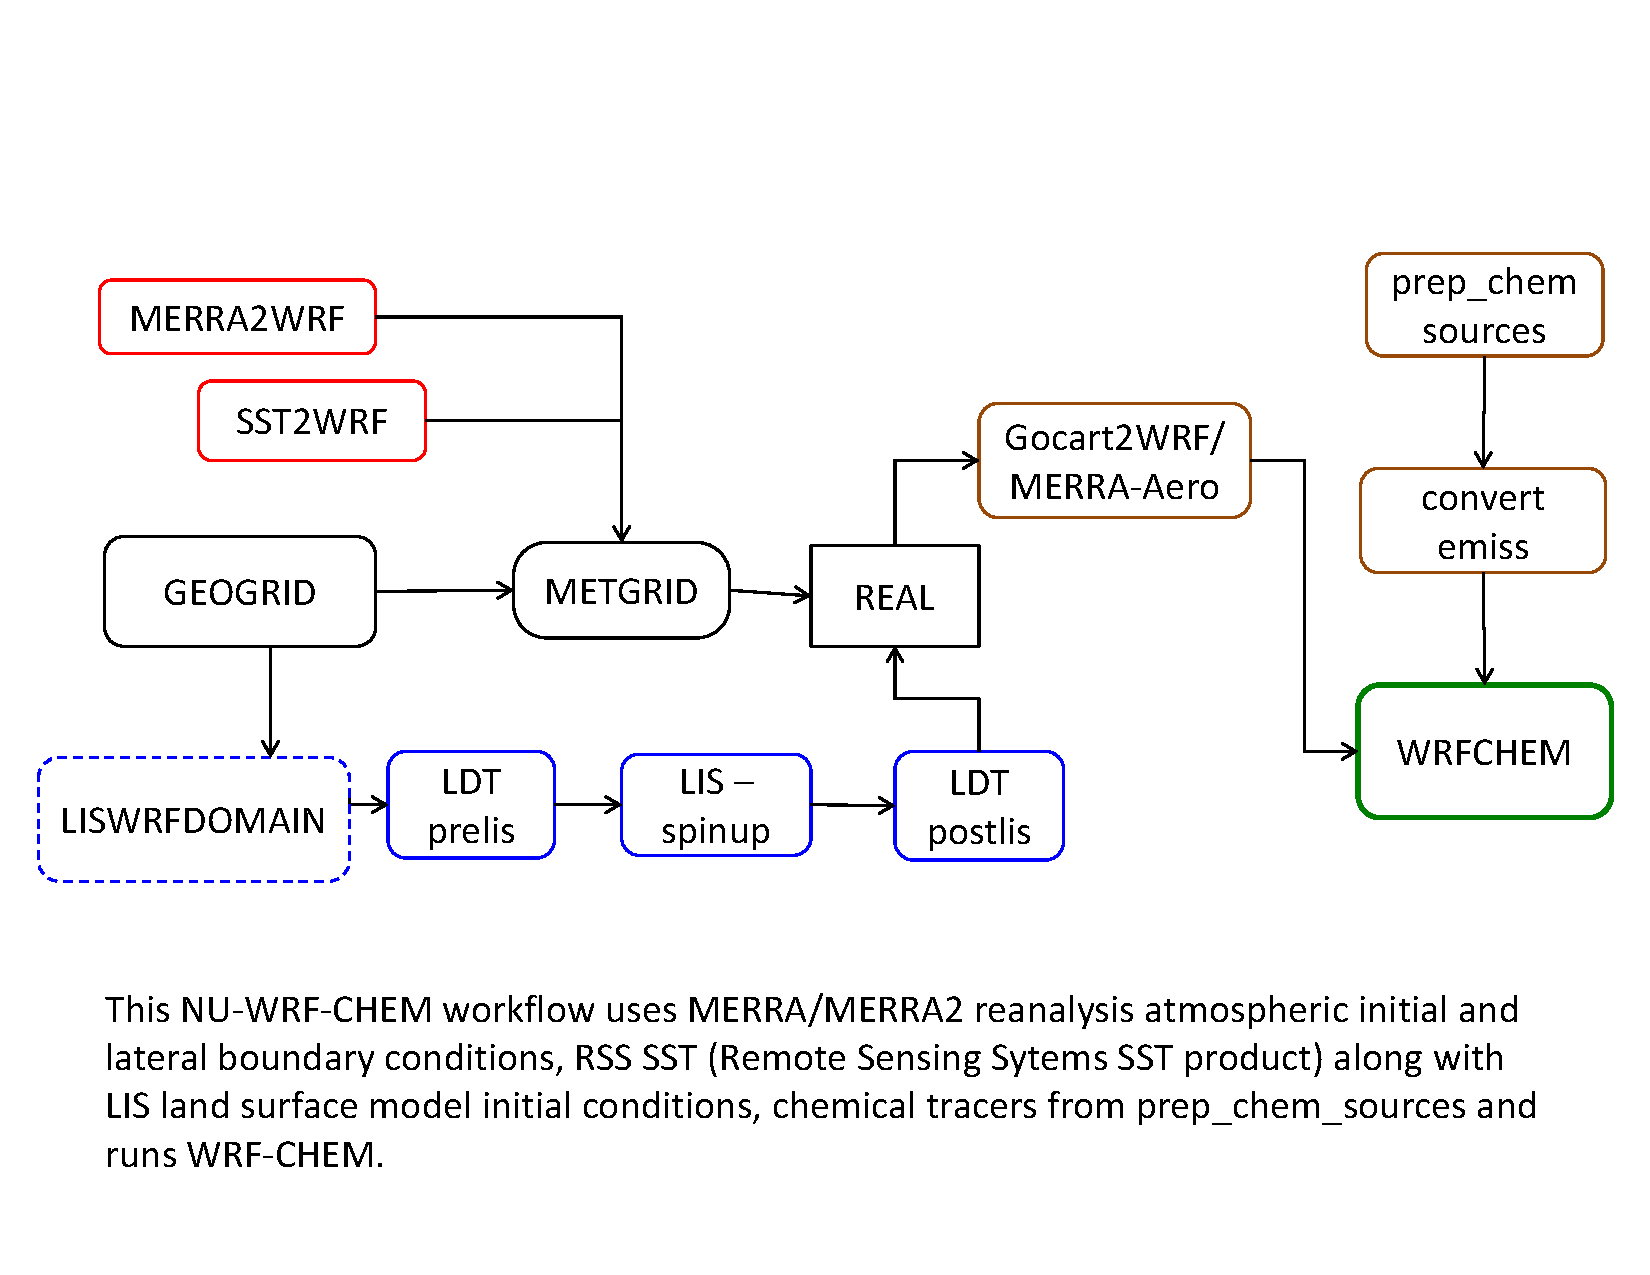
\includegraphics[scale=.38]{chemistry-workflow-2.pdf}
\end{figure}

\end{frame}

